\begin{multicols}{3}[\section{Bluetooth 4.0}]

\rhead{Autor: Thomas Schaffroth}
\lfoot{Letzte Bearbeitung: 17.04.2016}

\newrefsegment

\begin{boxedminipage}{\linewidth}
\begin{tabular}{p{2,1 cm}p{2.7 cm}}
\textbf{Steckbrief}& \\
\end{tabular}
\begin{tabular}{p{2,1 cm}|p{2.7 cm}}
      Einsatz seit & Juni 2010\\
      \hline
      Frequenz"-bereich  & \SI{2400}{\giga\hertz}\\
      \hline
      Datenrate & \SI{1}{MBit/s}\\
      \hline
      Verbreitung & Weltweit\\
      \hline
      Reichweite & \SI{10}{\metre}\\
\end{tabular}
\end{boxedminipage}
\par
%Source http://www.fh-bingen.de/fileadmin/user_upload/Lehrende/Kilsch_Dieter/internet/projekte/TedoSchStiUnits.pdf -> Seite 9 findet ihr alle verwendbaren Einheiten, wie:
%\SI{Zahl}{\mega\hertz} oder \SI{Zahl}{\mili\metre}
%Ich weiß ehrlich gesagt nicht welche Einheiten ihr im Text genau braucht, aber in dem Dokument und mit obigen Beispiel sollte es umsetzbar ein.
\subsection*{Überblick}
Die Bluetooth Technologie wurde im Jahr 1994 als drahtlose Alternative zu Datenkabeln entwickelt, indem man Daten über Funk übertrug. Bluetooth wurde als offener Standard entworfen, um Verbindungen und Zusammenspiel zwischen verschiedenen Produkten und Industrien möglich zu machen.\cite{Bluetooth_4.1} Beispiele für die Nutzung von Bluetooth im Alltag sind Freisprechanlagen für Smartphones im Auto, das Telefonieren über Bluetooth Headsets, das Hören von Musik über einen drahtlosen Lautsprecher oder die Übertragung von Daten zwischen zwei mobilen Geräten, uvm. In diesem Artikel werden zu Beginn die Architektur, das Übertragungsverfahren und die Rahmenstruktur von Bluetooth allgemein erläutert, da sich daran in der Spezifikation 4.0 nichts geändert hat. Anschließend wird auf die Neuerungen von Bluetooth 4.0 eingegangen.

\subsection*{Technische Erläuterungen}
\subsubsection*{Architektur der Bluetooth Technologie}
Die Verbindung zwischen Bluetooth Geräten erfolgt über ein Piconetz. Ein Piconetz ist ein Personal Area Network von Endgeräten, die sich über Bluetooth verbunden haben. Unter einem Personal Area Network versteht man ein Netz, das von Kleingeräten wie PDAs (Personal Digital Assistant) oder Mobiltelefonen ad hoc auf- und abgebaut werden kann. 

Ein Piconetz besteht aus einem Master-Knoten, bis zu sieben aktiven Slave-Knoten, die sich in einem maximalen Umkreis von 10 m befinden, und bis zu 255 geparkten Knoten. Dabei entspricht ein Knoten einem mobilen Gerät bzw. Teilnehmer. Geparkte Knoten sind Geräte, die der Master in einen Ruhezustand versetzt hat, um den Batterieverbrauch zu senken. In diesem Zustand wird ein Gerät nur durch eine Aktivierung des Masters wieder aktiv gesetzt. Darüber hinaus ist es möglich mehrere Piconetze über einen Bridge-Knoten zu verbinden. Es entsteht ein sog. Scatternetz (Abbildung 1). In einem Piconetz sind Slaves nicht eigenständig sondern warten auf Anweisungen durch den Master. Dieser steuert den Takt und entscheidet wer in welcher Zeitscheibe (Zeitintervall) Daten übertragen darf. Die Kommunikation geschieht dabei nie von Slave zu Slave sondern  immer über den Master-Knoten.\cite{Bluetooth_4.2}

\begin{Figure}
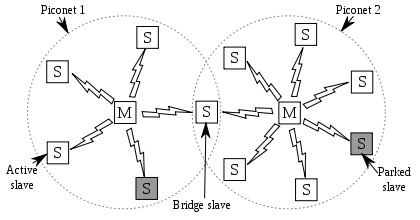
\includegraphics[width=\linewidth]{Kapitel/Bluetooth_4/Grafiken/piconetz.png}
\captionof{figure}{Zwei Piconetze druch einen Bridge-Knoten zu einem Scatternetz verbunden       \cite{Bluetooth_4.3} }
\label{fig:vorlage.vorlesungssaal}
\end{Figure}

\subsubsection*{Übertragungsverfahren}
Die Übertragung von Daten erfolgt über die Funkschicht. Bluetooth benutzt dafür das ISM-Band (Industrial, Scientific, Medical) im 2,4 GHz-Bereich. Daraus ergeben sich 79 Kanäle mit je einem MHz Bandbreite. Da jedoch das ISM-Band auch von anderen Netzen verwendet wird, kann es zu Störungen kommen. Um dies zu verhindern, wird bei Bluetooth eine Frequenzsprungtechnik mit Spektrumsspreizung verwendet. Es können bis zu 1600 Sprünge in der Sekunde über Zeitscheiben mit einer Dauer von 625 Mikrosekunden geschehen. In einem Piconetz springen alle Knoten zur gleichen Zeit und richten sich nach der Zeitscheibenvorgabe und Sprungfolge des Masters. Dazu kommt, dass sich Übertragungen früherer Versionen von Bluetooth und IEEE 802.11-Übertagungen gegenseitig zerstörten (Abbildung 2). Aus diesem Grund wurde die Frequenzsprungfolge so verändert, dass sie Kanäle auf denen andere Radio Frequenz-Signale existieren auslassen, um die schädlichen Interferenzen zu verkleinern. Diese Methode wird als adaptives Frequenzsprungverfahren (Abbildung 3) bezeichnet.\cite{Bluetooth_4.2}

\begin{Figure}
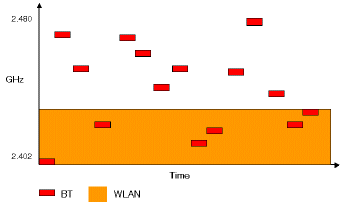
\includegraphics[width=\linewidth]{Kapitel/Bluetooth_4/Grafiken/kollisionen.png}
\captionof{figure}{Überlagerungen zwischen Bluetooth und IEEE 802.11\cite{Bluetooth_4.5} }
\label{fig:vorlage.vorlesungssaal}
\end{Figure}

\begin{Figure}
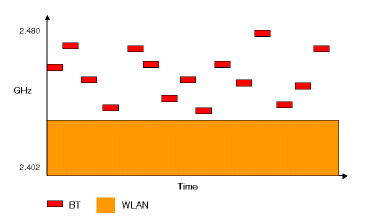
\includegraphics[width=\linewidth]{Kapitel/Bluetooth_4/Grafiken/frequenzsprung.png}
\captionof{figure}{Lösung durch das adaptive Frequenzsprungverfahren\cite{Bluetooth_4.5} }
\label{fig:vorlage.vorlesungssaal}
\end{Figure}

\subsubsection*{Rahmenstruktur}
Unter "Rahmen" versteht man in diesem Umfeld den Protokollrahmen, d.h. den Aufbau der Pakete, die zwischen Bluetooth Geräten ausgetauscht werden. Zwei wichtige Rahmenformate von Bluetooth sind in Abbildung 4 dargestellt, es gibt aber noch verschiedene andere. Den Anfang eines Rahmens bildet ein Zugriffscode, der den Master bestimmt. Dadurch können Slaves in der Reichweite von zwei Master-Knoten ermitteln, welche Daten für sie bestimmt sind. Es folgt ein 54-Bit-Header mit denselben Feldern, die auch für die MAC-Teilschicht im OSI-Modell typisch sind. 

Widmen wir uns kurz dem Header. Das Address-Feld gibt an, für welches Gerät im Piconetz der Rahmen bestimmt ist. Das Feld Type  spezifiziert den Rahmentyp (z.B. Polling), die Anzahl der Zeitscheiben, die der Rahmen umfasst, und die Art der Fehlerkorrektur, die im Datenfeld angewendet wird. Als nächstes stehen drei Flags. Das Flow-Bit kann von einem Slave-Knoten gesetzt werden, um anzuzeigen, dass sein Speicher voll ist, er also keine Daten mehr empfangen kann. Das Acknowledgement-Bit dient der Mitsendung einer Bestätigung in einem Rahmen. Das Sequence-Bit wird zur Nummerierung von Rahmen verwendet, um redundante Übertragungen zu erkennen. Schließlich folgt eine Prüfsumme von 8 Bit. 

Wenn der Rahmen mit Basisdatenrate gesendet wird, folgen auf den Header die Daten. Das Datenfeld kann abhängig davon über wie viele Zeitscheiben die Übertragung stattfindet von 0-2744 Bit lang sein. In dem Fall, dass der Rahmen mit erweiterter Datenrate gesendet wird, kann das Datenfeld bis zu zwei- oder dreimal so viele Bits besitzen. Den Daten ist nun ein Sicherheitsfeld und Synchronisationsmuster vorangestellt. Die Aufgabe des Synchronisationsmusters ist es, auf die schnellere Datenrate umzuschalten. Der Grund ist, dass der Adresscode und der Header mit Basisrate und nur die Daten mit erweiterter Datenrate gesendet werden. Üblicherweise werden Rahmen mit erweiterter Datenrate mit einem Trailer abgeschlossen.\cite{Bluetooth_4.2}

\begin{Figure}
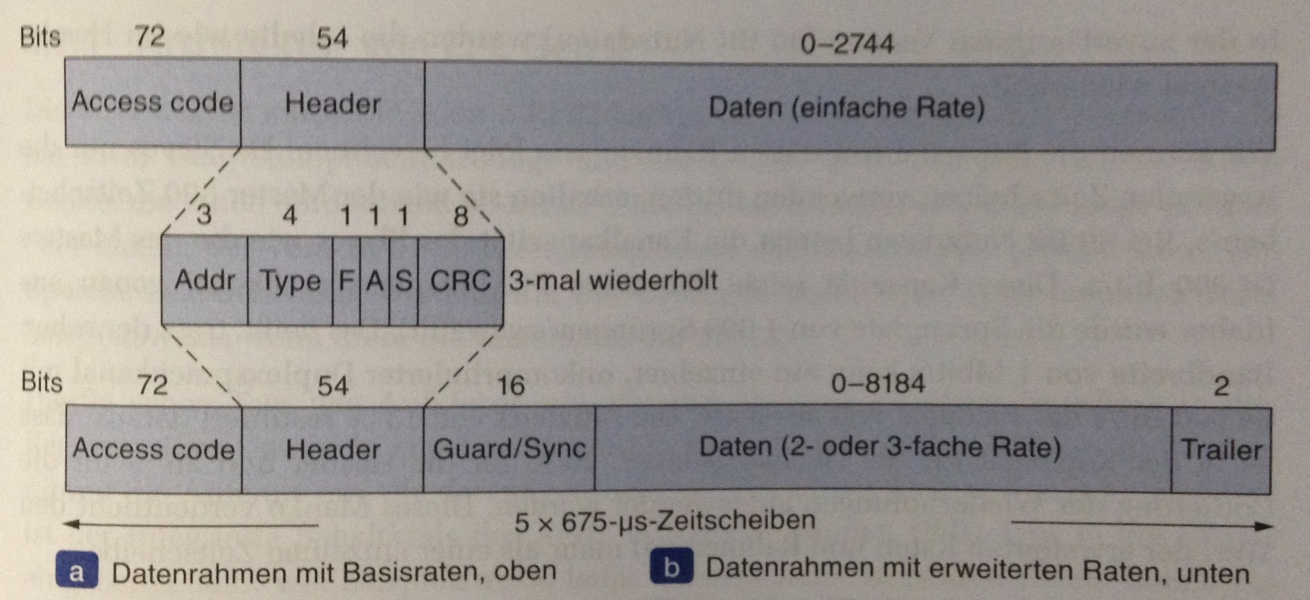
\includegraphics[width=\linewidth]{Kapitel/Bluetooth_4/Grafiken/rahmenstruktur.jpg}
\captionof{figure}{Überblick über die Rahmenstruktur in Bluetooth\cite{Bluetooth_4.2}
}
\label{fig:vorlage.vorlesungssaal}
\end{Figure}

\end{multicols}
\newpage
\section*{Historische Entwicklung}
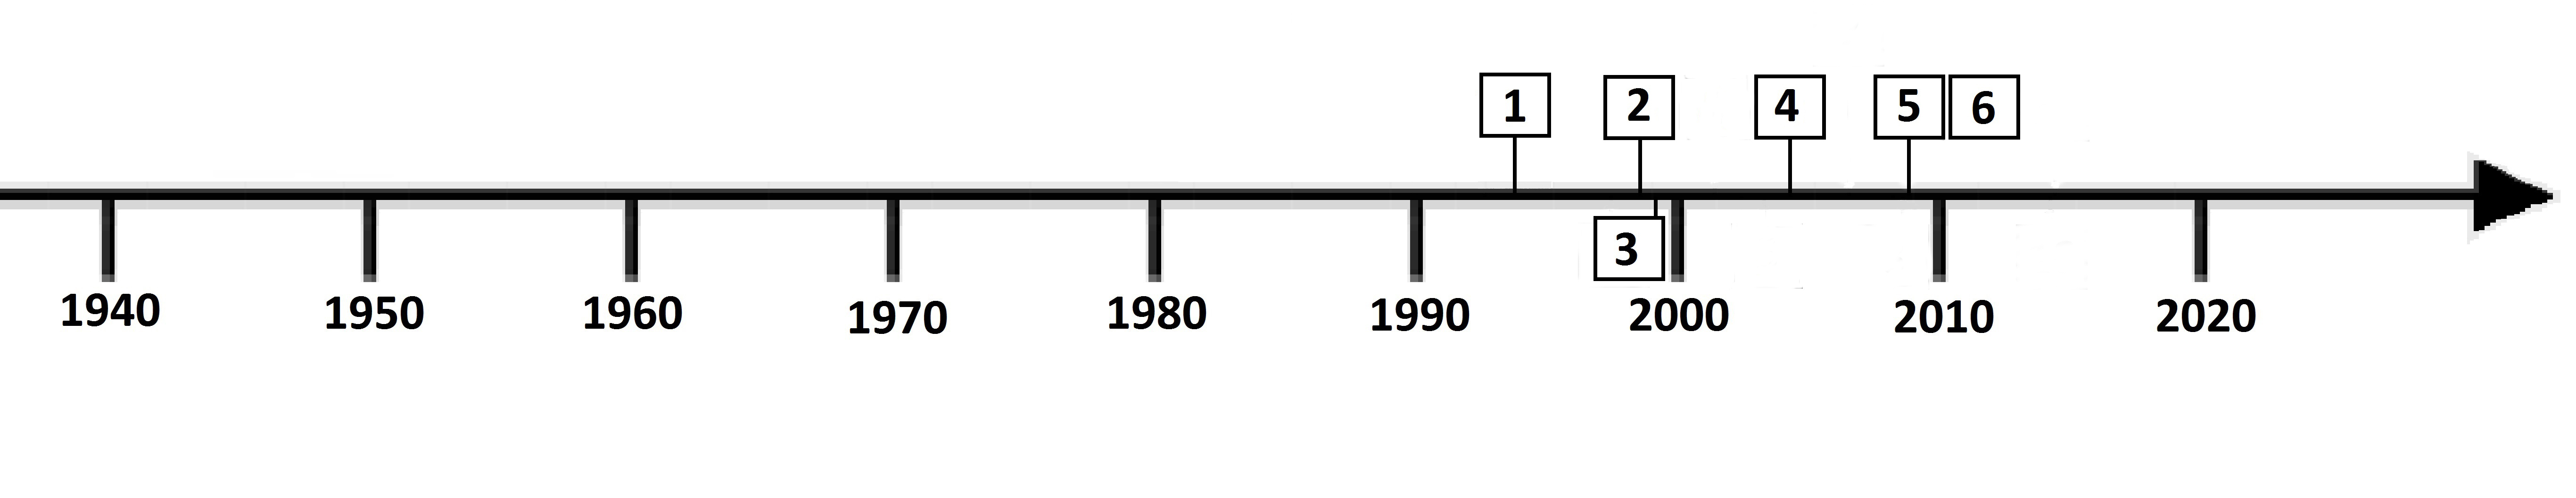
\includegraphics[width=\textwidth]{Kapitel/Bluetooth_4/Grafiken/zeitstrahl_bearbeitet}
\par
\noindent
\begin{tabular}{|p{1 cm}|p{3 cm}|p{13.55 cm}|}
	\hline
	Nummer & Datum & Entwicklungsschritte~\cite{Bluetooth_4.2}\\
	\hline
	1 & 1994 & Das Unternehmen L.M.Ericsson beginnt mit der Entwicklung einer Technologie für kabellose Verbindungen zwischen Mobiltelefonen und anderen Geräten.\\
	\hline
	2 & 1998 & Bildung der Bluetooth Special Interest Group (SIG) mit vier anderen Unternehmen, um einen drahtlosen Standard zur Verbindung von Rechnern und Kommunikationsgeräten zu spezifizieren. Die Prämisse dafür ware kostengünstige Funktgeräte mit niedrigem Strombedarf zu verwenden.\\
	\hline
	3 & Juli 1999 & Veröffentlichung von Bluetooth 1.0\\
	\hline
	4 & 2004 & Nachdem die Protokolle aus Version 1.0 stabil laufen werden diese mit höheren Datenraten zu Bluetooth 2.0 ergänzt.\\
	\hline
	5 & 2009 & Mit der dritten Version von Bluetooth werden in Kombination mit IEEE 802.11 Datenübertragungen mit höherem Durchsatz möglich\\
	\hline
	5 & Dezember 2009 & Veröffentlichung der Spezifikation für Bluetooth 4.0, die Niedrigenergiebetrieb inkludiert\\
	\hline
\end{tabular}
\par
\begin{multicols}{3}

\subsubsection*{Neuerungen von Bluetooth 4.0}
Man spricht bei Bluetooth in der Version 4.0 auch von Bluetooth Low Energie (LE). Der Name leitet sich davon ab, dass es sich um eine im Gegensatz zu seinen Vorgängern sehr stromsparende Version handelt. Dadurch ergeben sich nun auch Anwendungsmöglichkeiten auf Geräten bei denen dies bisher nicht möglich gewesen wäre, da einfach die Batterie für den längeren Betrieb von Bluetooth nicht ausgereicht hätte. Für die Chips von Bluetooth 4.0 reicht nur eine kleine Batterie aus, um längere Zeit arbeiten zu können. Low-Energy-Geräte ab Bluetooth 4.0 sind speziell für Anwendungen ausgelegt, die in größeren Intervallen kleine Datenmengen übertragen. Reine Low-Energy-Geräte sind beispielsweise Smartwatches, Sportsensoren oder Aktivitätstracker, die sich mit einem Smartphone koppeln. Bluetooth 4.0 ist allerdings nur bedingt zu früheren Versionen kompatibel. Ein Gerät, dass nur Bluetooth 4.x kennt, setzt bei seiner Gegenstelle ebenfalls Bluetooth 4.x voraus.\cite{Bluetooth_4.6}

\subsection*{Einsatz}
Die Bluetooth SIG spezifiziert Anwendungen, die unterstützt werden sollen und stellt für jede eine Reihe von Protokollen bereit. Es existieren eine ganze Reihe von Anwendungen auch „Profile“ genannt. Im Folgenden werden zunächst ausgewählte Profile und ihre Anwendungen vorgestellt, die nicht mit Bluetooth 4.0 spezifiziert wurden, sondern mit älteren Versionen. Diese wurden jedoch in der 4.0-Spezifikation übernommen und mit neuen Profilen ergänzt. Einige Profile sind für die Übertragung von Audio und Video vorgesehen. Ein Beispiel ist das Interkommunikationsprofil (ICP, INTP), welches es möglich macht zwei Telefone als Walkie-Talkies zu verbinden. Dazu kommen Headset- und Freisprechprofile, um Peripheriegeräte wie Headsets mit einer Basisstation zu verbinden. Andere Profile regeln das Streamen von Audio- und Videodaten in Stereoqualität beispielsweise von einem Handy auf einen tragbaren Lautsprecher oder von einer Kamera auf einen Fernseher. 

Außerdem existieren Profile zum Verbinden von Tastaturen und Mäusen an einen PC (HID), um ein Handy als Fernbedienung für einen Bluetooth-fähigen Fernseher zu verwenden oder Profile, die Netzbetrieb ermöglichen. Zu letzteren gehören zum Beispiel das PAN-Profil (Personal Area Networking) mit dem Bluetooth-Geräte ein Ad-hoch-Netz bilden können oder das DUN-Profil (Dial-Up Networking) durch das sich ein Notebook kabellos mit einem Handy verbinden kann, dass ein Modem enthält. Erwähnenswert ist das Generic-Attribute-Profil (GATT), dass für die neue Version Bluetooth 4.0 spezifiziert wurde. Es wird als Master-Profil für andere Profile verwendet, um kleine Datenmengen energieeffizient zu übertragen. \cite{Bluetooth_4.2} Eine vollständige Übersicht aller bisherigen Profile inklusive GATT mit ihren Einsatzgebieten kann hier gefunden werden: https://de.wikipedia.org/wiki/Bluetooth-Profile.

\subsection*{Anbieter und Gremien}
Für die Bluetooth-Technologie einschließlich der Version 4.0 ist die Bluetooth SIG (Special Interest Group) zuständig. Diese wurde 1998 von 5 Unternehmen gegründet und war im März 2015 bereits eine Interessengemeinschaft von mehr als 8000 Unternehmen, die bei der Entwicklung und Verbreitung der Technologie zusammenwirken. Die Bluetooth SIG ist darüber hinaus auch der Eigentümer des Bluetooth-Zeichens und Herausgeber der Bluetooth-Spezifikation.\cite{Bluetooth_4.4}

\subsection*{Ausblick}
Die Bluetooth-Technologie ist heute für das kabellose 
Verbinden von verschiedenen Geräten unerlässlich geworden. 
Das gilt sowohl für die älteren Spezifikationen als auch für 
Bluetooth 4.0 durch das völlig neue Einsatzgebiete möglich werden. 
Dies betrifft vor Allem den Betrieb auf kleinen Geräten für die 
Bluetooth-Anwendungen bisher aufgrund des hohen Energieverbrauchs
nur bedingt nützlich waren. Meiner Meinung nach ist die Technologie
von Bluetooth sehr interessant und es ist lohnenswert sich damit einmal
genauer zu befassen zumal fast jeder von uns Bluetooth schon benutzt hat. 
Darüber hinaus bleibt es spannend zu verfolgen inwiefern sich Bluetooth 4.0 
und seine Einsatzgebiete in den nächsten Jahren entwickeln werden.
\printbibliography[segment=3,heading=subbibliography]
\end{multicols}

\newpage
